\chapter{Algorithms}

\section{General algorithms}

\subsection{Peak extraction}

In order to use the \gls{cir} recovered either in the simulation or from the experimental set-up, those need to be processed. The major objective is to retrieve the different peaks that originates from the physical anchor and the \gls{vas}. Unfortunately, the \gls{cir} obtained is not as simple as shown in Fig. \ref{fig:UWB_MPC_Theo}. In order to obtain the same results, one would need some antennas with an infinite bandwidth\footnote{In order to obtain Dirac peaks, one need an infinite bandwidth since the $\delta(t) \xrightarrow{\mathscr{F}} 1 $}, a "clean" room and to receive to the receiver side only the rays coming from the \gls{los} or reflected once.
\vspace{2mm}

\begin{figure}[H]
\centering
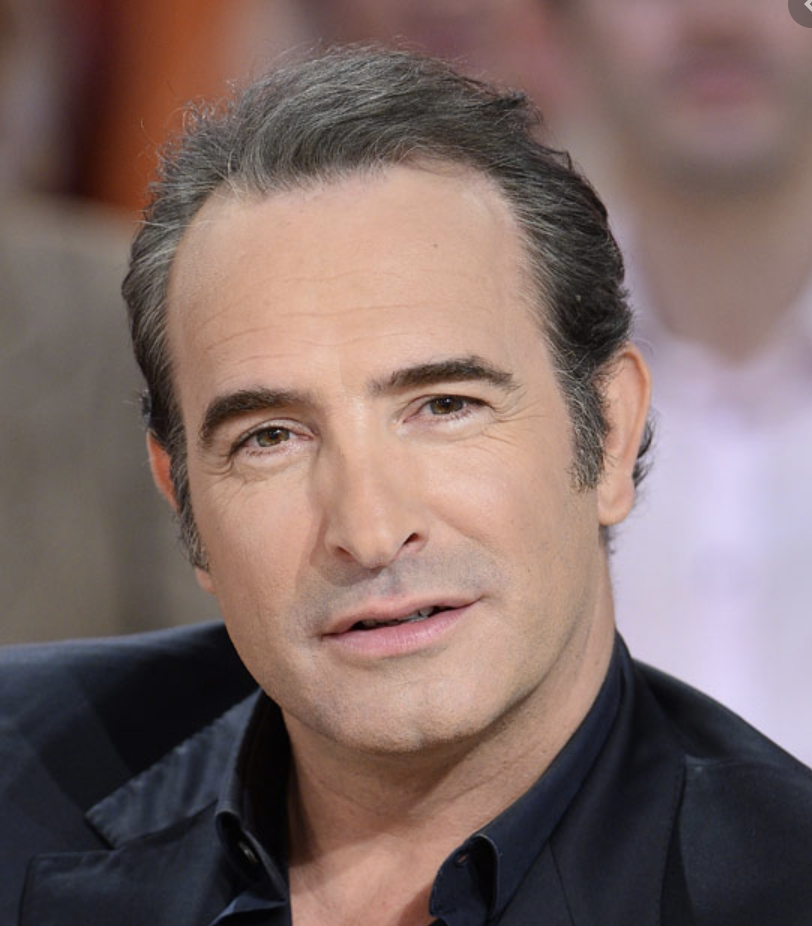
\includegraphics[width=.2\linewidth]{Images/Temporary_pic.png}
\label{fig:cir_example}
\caption{CIR example.}
\end{figure}

The \gls{cir} shown for Fig. \ref{fig:cir_example} has been generated in a rectangular cluttered room of 15 over 10m, filled with furnitures. The selected bandwidth is the same as for the experimental set-up : 499.2MHz. The positions of the tag have been kept the same as in Fig. \ref{fig:cir_ex1}. As one can observe on Fig. \ref{cir}, getting the different peaks is not as trivial.

\section{Hard localization algorithm}



\color{red}
\section{ALGOS UTILES (SPEED, DATA EXTRACTION}
\color{black}

\section{Speed-Up Algorithms}

\subsection{Speed-Up 1}

The aim of this algorithm is to speed up the locating process by reducing the number of needed computations. To achieve this, the \gls{cir}, that needs to be computed at each location, is only computed in a reduced set of possible position for the tag.
\vspace{2mm}

Using the \gls{sdstwr}, the \gls{tof} of the signal between the tag and the anchor can be computed\footnote{In the simulation, it will be assumed to be extracted from the \gls{cir}}. Based on this \gls{tof}, a circle can be traced with the center on this anchor and the radius being the estimated distance deduced from the \gls{tof}. In theory, the tag is supposed to be located on this circle, but due to the discretization and errors on the \gls{tof}, a margin is taken to get the set of possible locations. This margin resides in the two orange circles, that can be observed on Fig. \ref{fig:speedup_1}.
\vspace{2mm}

\begin{figure}[H]
\centering
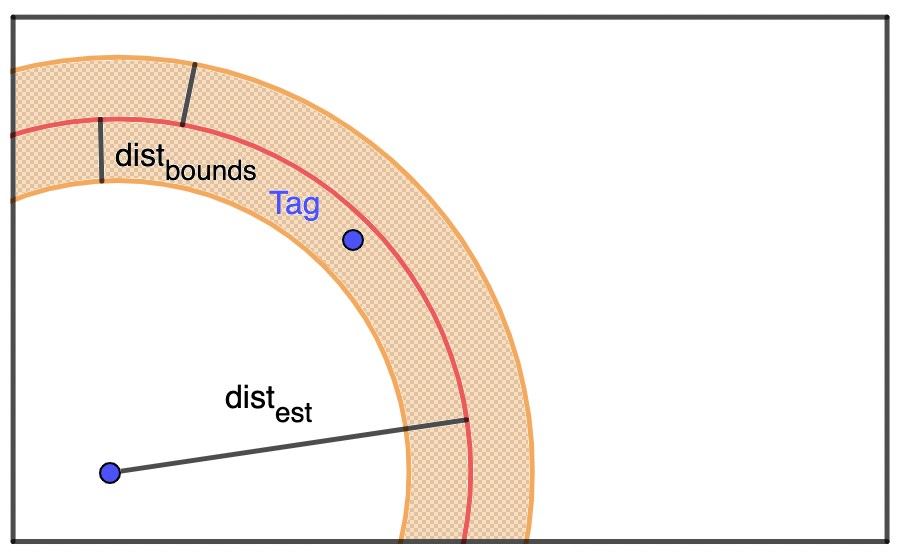
\includegraphics[width=.65\linewidth]{Images/algo_1.png}
\caption{Example of algo 1}
\label{fig:speedup_1}
\end{figure}

From the position inside those boundaries, a mask matrix representing all the position of the room is filled with ones for the position inside of the orange zone. The other positions are left to zero. Later, this mask is used to reduce the computations since only the values associated with a one will be tested.

\subsection{Speed-Up 2}

Choix des ancres en utilsant l'algorithme numéro 1

\color{red}
\section{LOCATION METHOD, HARD VS SOFT}
\color{black}

Parler des deux manière de fournir une position.

\section{Pos Finder}

This locating system is based on the idea of trilateration and tries to mimic it. Using three peaks, it tries to associate those with the anchor and two virtual anchors to find an intersection point as in the Fig. \ref{fig:triangulation}.

The theory behind this algorithm relies on the fact that the three first algorithm

- Mettre le schéma de l'antenne qui est dans un coin, et des 4 zones qui se dessinent
	- Ne pas oublier le cas où l'on a 6 zones en fait (dans les pièces rectangulaires)
- Expliquer qu'on va tester toutes les possibilités 2 à 2, mais qu'on peut éliminer certaines avec l'algo speed 2.
- Expliquer que si ça ne marche pas 2à2, on test les cas où les rayons qui arrivent sont confondus.


Les problèmes de cet algo proviennent en partie des symmétries, mais on verra ça dans la simulation, ne pas encore en parler mtn

\section{CIR MSE}

Pour la forme de la CIR, bien expliquer pourquoi ça ne marche pas vraiment. Même en atténuant les autres pics de la même manière que le pic principal. Parce que la réponse qu'on reçoit peut avoir un LoS légèrement plus obstrué que le reste, ou vice versa. Ca marche bien dans la simulation, mais ça sera probablement moins efficace IRL.

\section{Time MSE}

Méthode préférée à CIR
